% !TEX root = ../notes_3dprinting.tex
% Chapter 1: Quickstart -- install, bind, and print one known part
%%%%%%%%%%%%%%%%%%%%%%%%%%%%%%%%%%%%%%%%%%%%%%%%%%%%%%%%%%%%%%%%%%%%%%

\index{quickstart}\index{Bambu P1S}\index{Bambu Studio}
\chapter{Quickstart}
\printchapterversion{01_quickstart}

\vspace{1.5em}
\section{Log In}

\newthought{Bambu Studio is the companion software.} Download it and
install it with the defaults. On first start, create a free Bambu Lab
account or sign in with a preexisting one.
\marginnote{\newthought{Download.}
\url{https://bambulab.com/en/download/studio}}

\section{Bind the Printer}

\marginnote{\newthought{If the printer is already bound to someone else,}
it will not offer itself for binding. Log the previous user out.
On the printer screen open the gear \icongear{}, then
\texttt{Account}, and log out. Then bind it.}

\index{binding}\newthought{The P1S is bound to exactly one account at a time.} With your
laptop on the same network as the printer, open the \texttt{Device} tab in
Bambu Studio, pick the P1S from the list of nearby printers, and confirm the
request on the printer screen, on first login usually via a code.




\section{The Printing}

\begin{marginfigure}
  \centering
  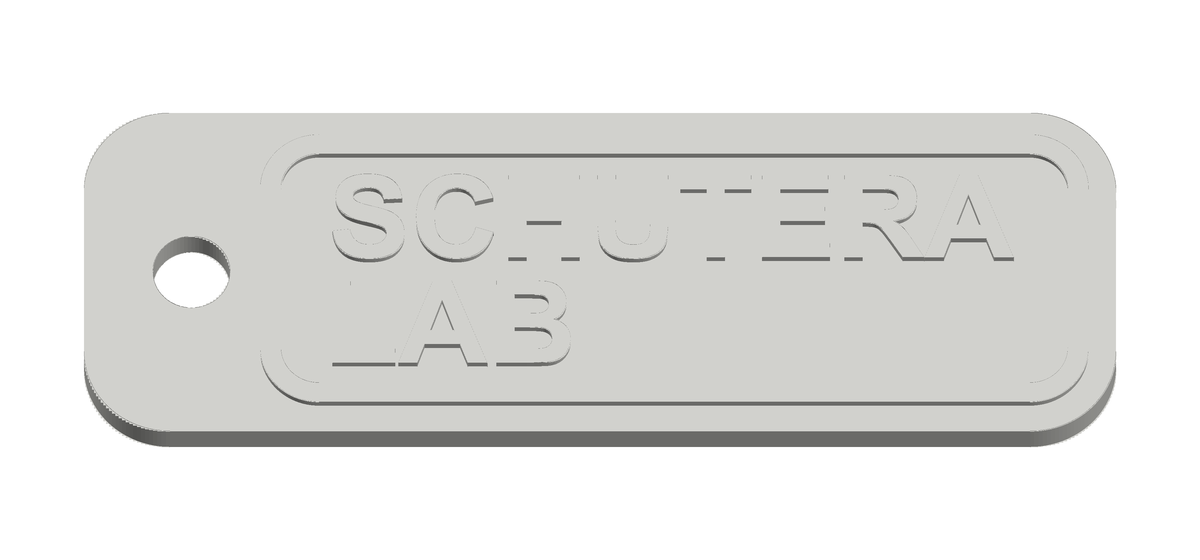
\includegraphics[width=0.75\marginparwidth]{figures/testprint.png}
  \caption{The test part. The flat base sanity checks the first layer, the hole
  checks dimensions, the letters and the rim check small features.}
\end{marginfigure}

\index{test part}\newthought{A test part for your first print} is provided to the right. Ours is a Schutera Lab
keyring tag: $60 \times 20 \times 2.4$~mm, a 4.5~mm hole that takes a
standard split ring, and lettering and a border rim raised 0.6~mm, which
is three layers at the standard layer height. \texttt{testprint.stl} lives
next to this PDF and in the course repository, and may be shared and used freely.
\marginnote{\newthought{Download.}
\url{https://github.com/Quillstacks/LectureMaterial/raw/main/lecturenotes/notes_3dprinting/testprint.stl}}
If you want to pick your own first print, choose something small, flat, and simple.
\marginnote{\newthought{Bringing your own parts later?} Prefer a
\texttt{.3mf} over an \texttt{.stl}: it carries units, orientation, and
settings with it.}
\marginnote{\newthought{No outside filament.} Print only with
material provided by the lab.}

\index{slicing}\index{nozzle profile}\newthought{Slice.} In the \texttt{Prepare} tab
choose \texttt{Bambu Lab P1S} with the \texttt{0.4 nozzle} profile.
\marginnote{\newthought{Nozzle profiles can change.} We feature the
\texttt{0.4 nozzle} here because it allows us to
print TPU (see p. \pageref{ch:tpu}).} Drag \texttt{testprint.stl} onto the plate. 
Choose the AMS slot\index{AMS} you intend
to print from and confirm the plate type is \texttt{Textured PEI Plate}\index{textured PEI plate}.
Then press \texttt{Slice} and read the preview. This will tell you about grams and job duration
and is a good menas for a sanity check.

\index{first layer}\newthought{Check the physical plate before you send.} Clean, dry, seated flat on the
magnets, no fingerprints where the part will land. Then send the job. The
machine spends a few minutes heating and leveling before the first line of
plastic goes down.

\marginnote{\newthought{Watch the first layer finish.} before you walk
away. If it is not down cleanly, stop the job there. These printers get hot and need attendance, so never walk away too far anyways. 
Weekend and overnight jobs need to be permitted by Lab Staff aka a Professor.}

\index{plate}\newthought{Let the plate cool before you touch the part.} PLA
releases its grip as the plate cools; then flex the plate rather than
prying the part. The magnetic lock-on feature allows you to take the plate
out of the printer. Put the plate back, and close the door.

\marginnote{
  \medskip

Scan the code
and send a mail stating your project, faculty and what filament you used up (in g).
\\
\medskip
\null\hfill\qrcode[height=1.0cm]{mailto:schutera@dhbw-ravensburg.de?subject=3D\%20Print\%20Log\&body=Project\%3A\%20\%0AMaterial\%20used\%20(g)\%3A\%20}
\medskip}

\newthought{Leave the machine the way you found it.} If you are done for
the day, make sure the lamp is off, the surrounding of the machine and its inside are tidy and clean.
It is okay to turn off the printer entirely.
